\begin{frame}{Neural Networks - Processing information}
\begin{tabular}{p{5cm}|p{5cm}}
    \begin{figure}
    	
\includegraphics[scale = 0.09]{brain}
    \end{figure}
    & 
    \begin{figure}
    	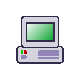
\includegraphics[scale = 1.4]{machine}
    \end{figure} \\
  \multicolumn{1}{c|}{Humam senses} & \multicolumn{1}{c}{Input variables} \\
    \begin{itemize}
        \item Extraction of relevant info
        \item Impossible for machines
    \end{itemize}
    & 
    \begin{itemize}
      \item Preprocessed by user
      \item {e.g.} kinematic variables
    \end{itemize} \\
\multicolumn{1}{c|}{Human brain} & \multicolumn{1}{c}{Net of nodes} \\
    \begin{itemize}
        \item Web of neuron cells
        \item Input from surrounding cells
        \item Single combination $\rightarrow$ action
    \end{itemize}
    & 
    \begin{itemize}
      \item Nodes = simple processors
      \item Connected by linear function
      \item Combination forms non-linear model
    \end{itemize} 
 \end{tabular}
\end{frame}


\begin{frame}{Neural network structure}
\begin{figure}
\centering
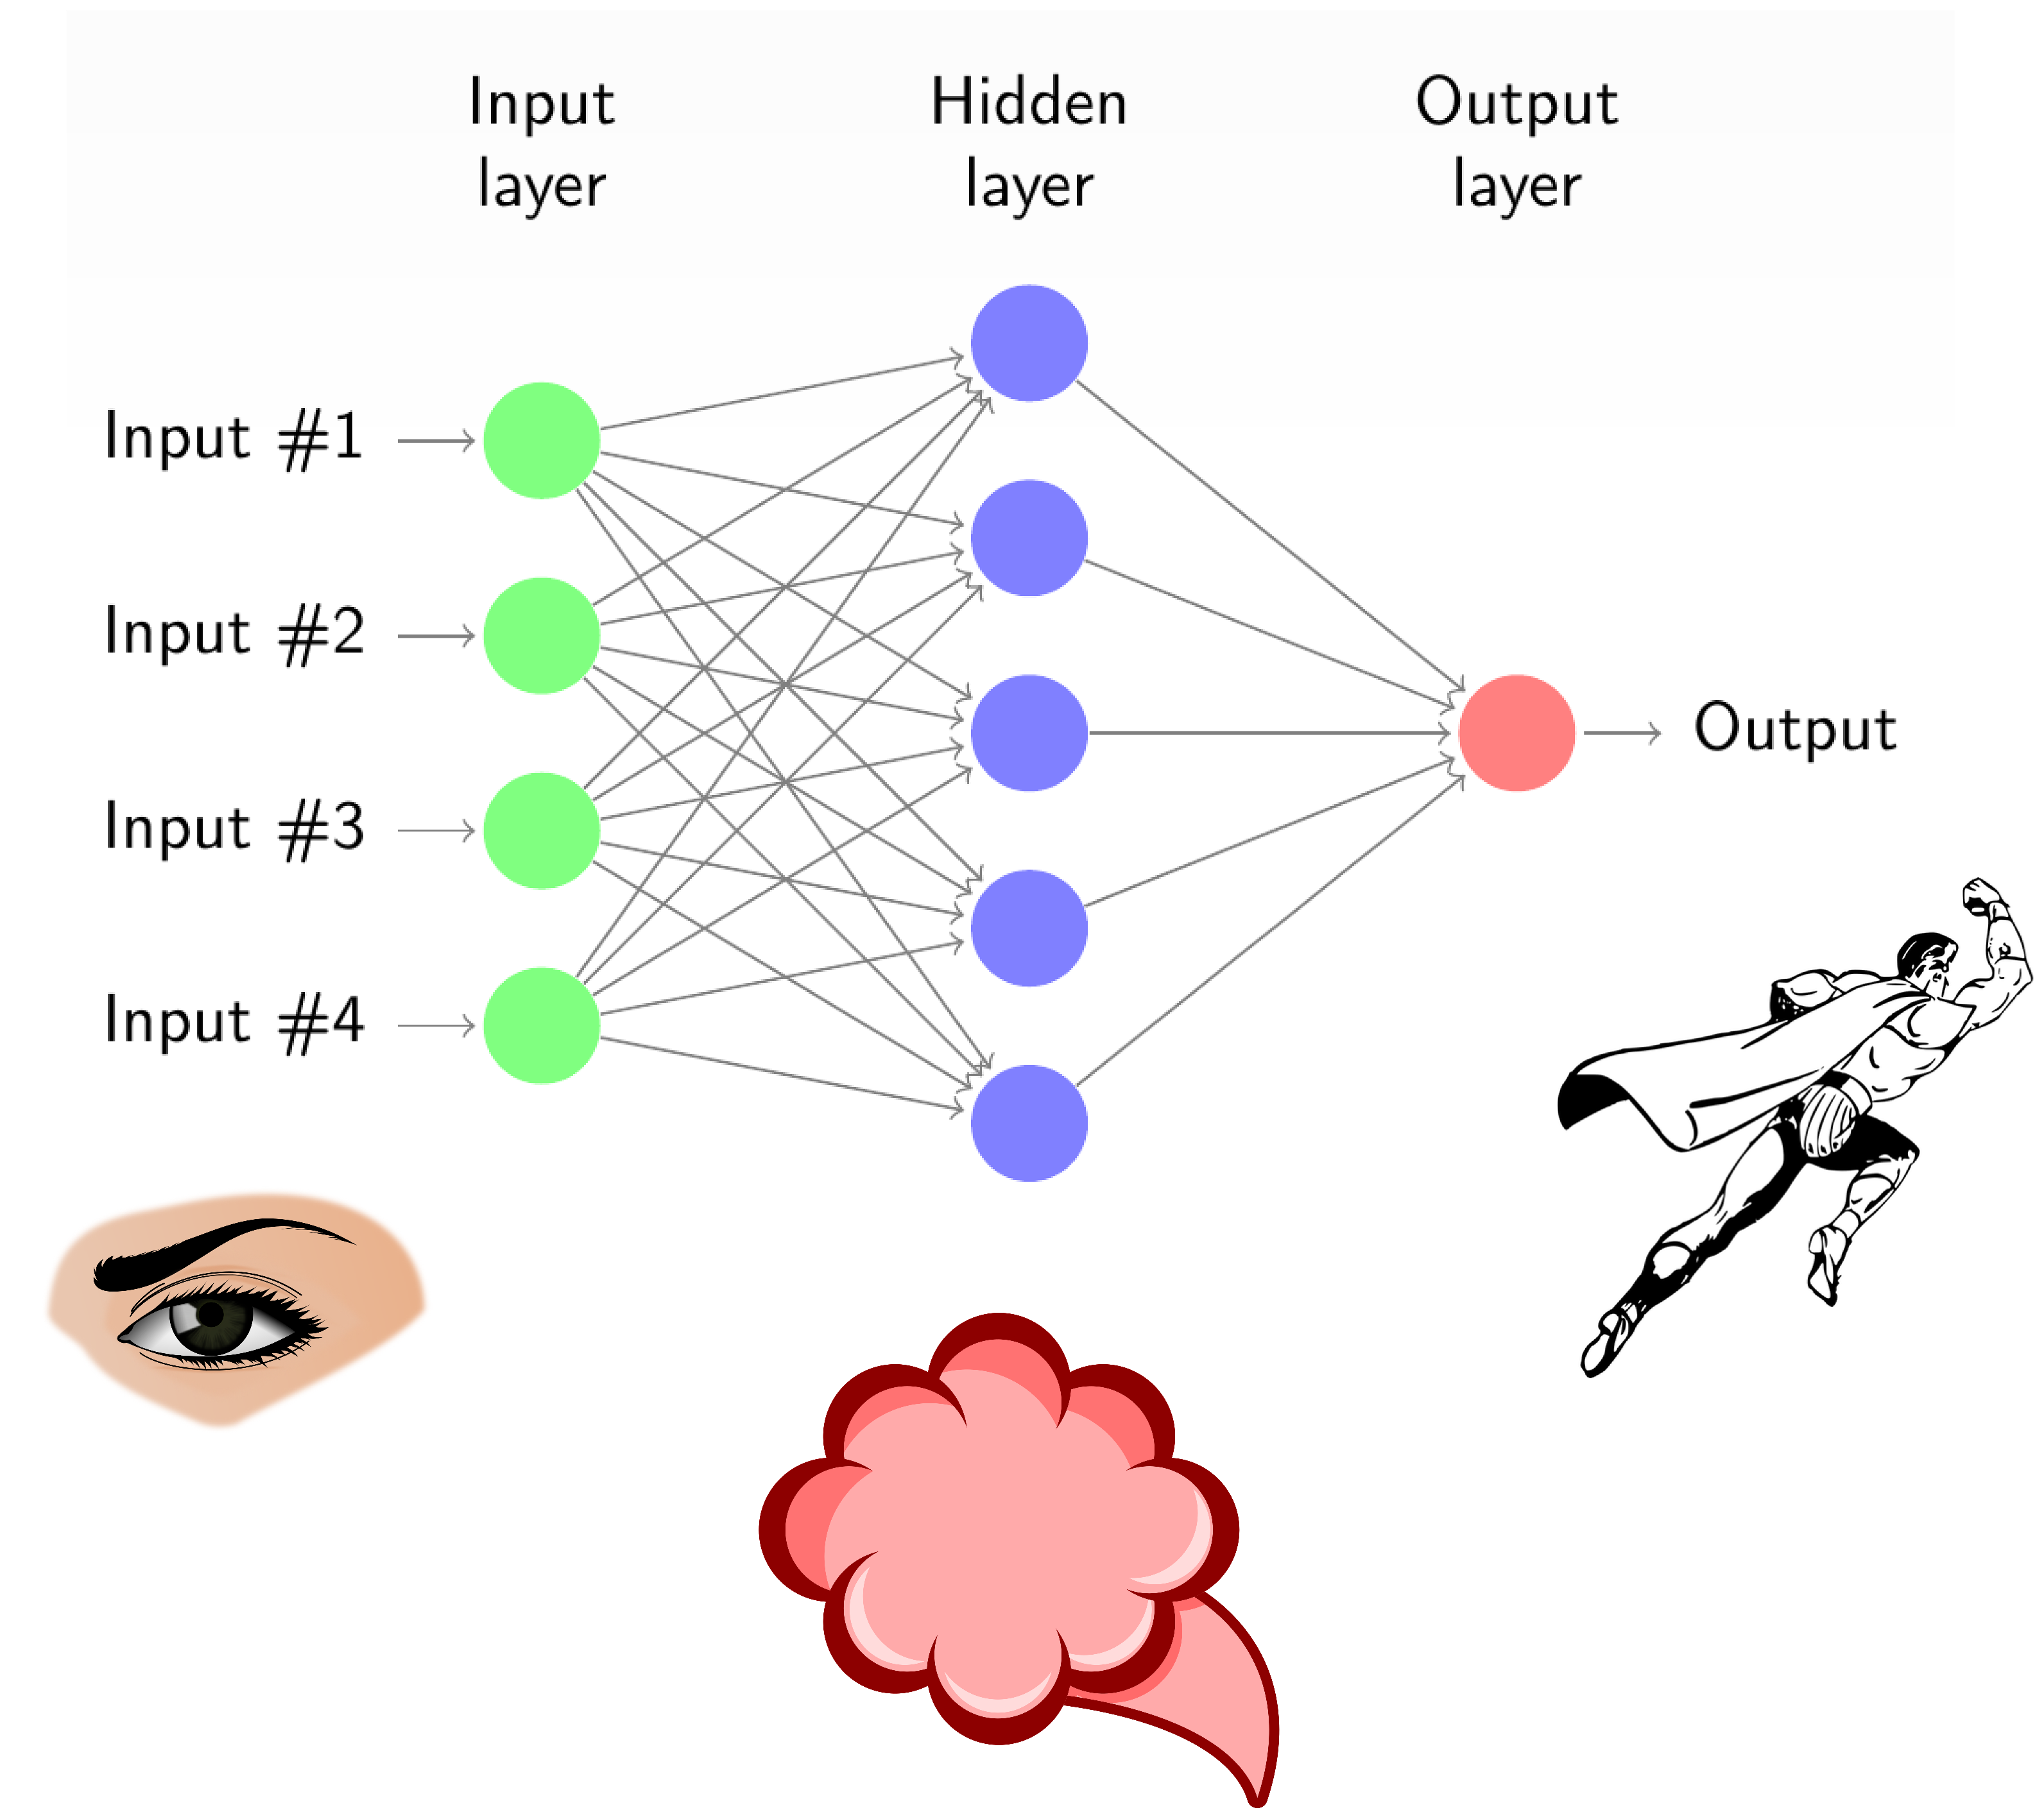
\includegraphics[width=0.8\textwidth]{net_structure}
\end{figure}
\end{frame}

\begin{frame}{Neural Networks - Choosing the next step}
\begin{tabular}{p{5cm}|p{5cm}}
    \begin{figure}
    	
\includegraphics[scale = 0.09]{brain}
    \end{figure}
    & 
    \begin{figure}
    	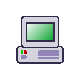
\includegraphics[scale = 1.4]{machine}
    \end{figure} \\
  \multicolumn{1}{c|}{Evaluation of an action} & \multicolumn{1}{c}{Loss function} \\
    \begin{itemize}
        \item Simple perceptions: pain, satisfaction
        \item Expectation
    \end{itemize}
    & 
    \begin{itemize}
      \item Supervised learning: compare to the desired outcome
      \item Loss = estimator for quality
    \end{itemize} \\
\multicolumn{1}{c|}{Decision for a next step} & \multicolumn{1}{c}{Optimisation} \\
    \begin{itemize}
        \item Trial and error
        \item Learning from experience
    \end{itemize}
    & 
    \begin{itemize}
      \item Back-propagation impact of parameters' on the loss
      \item Adjust parameters to minimise plot
    \end{itemize} 
 \end{tabular}
\end{frame}

\begin{frame}{Hyperparameter optimisation}
    \begin{block}{What is a hyperparameter?}
        \begin{itemize}
            \item During the learning process the neural network optimises its internal parameters
            \item Some parameters are still set by the user according to the task of the network
            \item These are called hyperparameters
        \end{itemize}
        
    \end{block}
    \begin{block}{How does one optimise the choice?}
        \begin{itemize}
            \item Neural networks provide several metrics to estimate result and performance
            \item To optimise the hyperparameters one usually runs several configurations to find a good set of parameters
        \end{itemize}
    \end{block}
\end{frame}


\begin{frame}{Concepts of evolutionary network optimisation}
    \begin{block}{Choosing a start}
        \begin{itemize}
            \item Randomly choose a set of values for each hyperparameter
            \item Combine the random selection to create a set of network configurations
        \end{itemize}
    \end{block}
    \begin{block}{Evaluating a start}
        \begin{itemize}
            \item Run the networks for a small number of epochs
            \item Use networks' metrics to evaluate the performance
        \end{itemize}
    \end{block}
    \begin{block}{Choosing a next step}
        \begin{itemize}
            \item Rank networks by their metrics
            \item Reuse, mate and mutate networks
        \end{itemize}
    \end{block}
\end{frame}

\begin{frame}{The initial generation}
    \begin{block}{Current setup}
        \begin{itemize}
            \item Choose a random set of hyperparameters from a range of paramters set by the user
            \item Create a set of neural networks from all possible combinations
        \end{itemize}
    \end{block}
    \begin{block}{Planned}
        \begin{itemize}
            \item Draw each hyperparameter from a fitting distribution
            \item Restrict the number of combinations based on the hyperparameter
        \end{itemize}
    \end{block}
\end{frame}

\begin{frame}{Evaluating a generation}
    \begin{block}{Current setup}
        \begin{itemize}
            \item Evaluate all networks based on a metric of choice
            \item The metric of choice can be simply the AUC
            \item Save the $x$ best configuration
        \end{itemize}
    \end{block}
    \begin{block}{Planned}
        \begin{itemize}
            \item Test and combine different metrics
            \item Implement different metrics with regard to early stopping
        \end{itemize}
    \end{block}
\end{frame}

\begin{frame}{Breeding the next generation}
    \begin{block}{Current setup}
        \begin{itemize}
            \item Always keep the best configuration
            \item Recombine the $\lambda$ best configurations
            \item Recombine the $\lambda$ best generations again and vary $\mu$ hyperparameters
        \end{itemize}
    \end{block}
    \begin{block}{Planned}
        \begin{itemize}
            \item Include more hyperparameters
            \item Specify different variation probabilities and values for different hyperparameters
        \end{itemize}
    \end{block}
\end{frame}

\begin{frame}{Summary of the optimisation process}
    \begin{columns}
    \begin{column}{0.5\textwidth}
        \begin{itemize}
            \item Survival of the fittest: Keep the best setup
            \item Recombination: Reuse the best hyperparameters for the next batch
            \item Variation: Randomly change the hyperparamters to avoid local minima and bias
        \end{itemize}
    \end{column}
    \begin{column}{0.5\textwidth}
        \begin{figure}
            \centering
            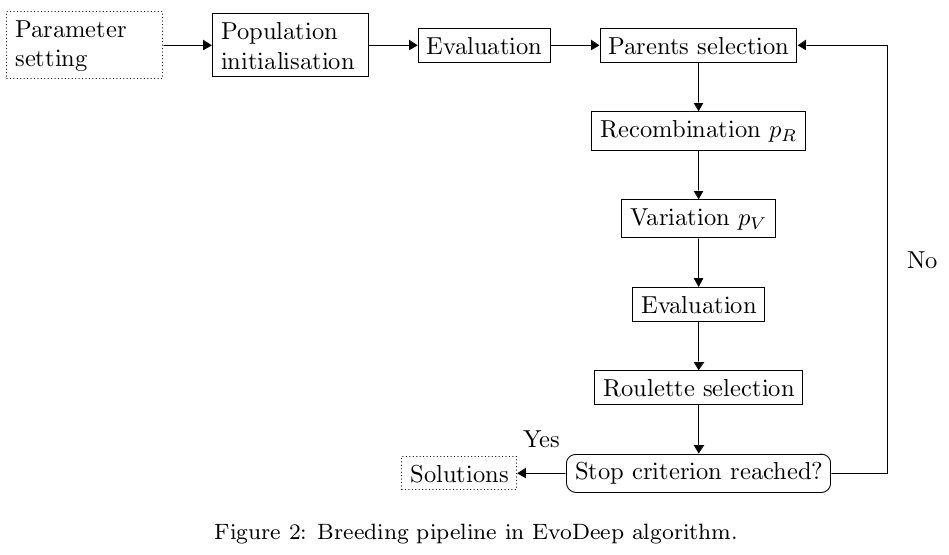
\includegraphics[width=\textwidth]{breed.png}
            \caption{\cite{naranjo}}
        \end{figure}
    \end{column}
    \end{columns}
\end{frame}